
\documentclass[twoside,twocolumn]{article}

\usepackage{blindtext} % Package to generate dummy text throughout this template 

\usepackage[sc]{mathpazo} % Use the Palatino font
\usepackage[T1]{fontenc} % Use 8-bit encoding that has 256 glyphs
\linespread{1.05} % Line spacing - Palatino needs more space between lines
\usepackage{microtype} % Slightly tweak font spacing for aesthetics

\usepackage[english]{babel} % Language hyphenation and typographical rules

\usepackage{graphicx}
\usepackage[hmarginratio=1:1,top=32mm,columnsep=20pt]{geometry} % Document margins
\usepackage[hang, small,labelfont=bf,up,textfont=it,up]{caption} % Custom captions under/above floats in tables or figures
\usepackage{booktabs} % Horizontal rules in tables

\usepackage{lettrine} % The lettrine is the first enlarged letter at the beginning of the text

\usepackage{enumitem} % Customized lists
\setlist[itemize]{noitemsep} % Make itemize lists more compact

\usepackage{abstract} % Allows abstract customization
\renewcommand{\abstractnamefont}{\normalfont\bfseries} % Set the "Abstract" text to bold
\renewcommand{\abstracttextfont}{\normalfont\small\itshape} % Set the abstract itself to small italic text

\usepackage{titlesec} % Allows customization of titles
\renewcommand\thesection{\Roman{section}} % Roman numerals for the sections
\renewcommand\thesubsection{\roman{subsection}} % roman numerals for subsections
\titleformat{\section}[block]{\large\scshape\centering}{\thesection.}{1em}{} % Change the look of the section titles
\titleformat{\subsection}[block]{\large}{\thesubsection.}{1em}{} % Change the look of the section titles

\usepackage{fancyhdr} % Headers and footers
\pagestyle{fancy} % All pages have headers and footers
\fancyhead{} % Blank out the default header
\fancyfoot{} % Blank out the default footer
\fancyhead[C]{Joel Stuart $\bullet$ August 2016 $\bullet$ COSC3500 $\bullet$ Project Milestone One} % Custom header text
\fancyfoot[RO,LE]{\thepage} % Custom footer text

\usepackage{titling} % Customizing the title section

\usepackage{hyperref} % For hyperlinks in the PDF

%----------------------------------------------------------------------------------------
%	TITLE SECTION
%----------------------------------------------------------------------------------------

\setlength{\droptitle}{-4\baselineskip} % Move the title up

\pretitle{\begin{center}\Huge\bfseries} % Article title formatting
	\posttitle{\end{center}} % Article title closing formatting
\title{Elastic Collisions in Two Dimensions COSC3500 Project Milestone 1} % Article title
\author{%
	\textsc{Joel Stuart - 43203714} \\[1ex] % Your name
	\normalsize University of Queensland \\ % Your institution
	\normalsize \href{mailto:joel.stuart@uq.net.au}{joel.stuart@uq.net.au} % Your email address
	%\and % Uncomment if 2 authors are required, duplicate these 4 lines if more
	%\textsc{Jane Smith}\thanks{Corresponding author} \\[1ex] % Second author's name
	%\normalsize University of Utah \\ % Second author's institution
	%\normalsize \href{mailto:jane@smith.com}{jane@smith.com} % Second author's email address
}
\date{\today} % Leave empty to omit a date
\renewcommand{\maketitlehookd}{%
	\begin{abstract}
		\noindent This report investigates a serial implementation of a multi-bodied simulation of elastic collisions in two dimensions. It details the algorithm used to implement the simulation and the assumptions and limitations the algorithm makes. It also discusses the performance of the implementation at varying problem sizes and comments on the verification methods of the implementation.
	\end{abstract}
}

%----------------------------------------------------------------------------------------

\begin{document}
	
	% Print the title
	\maketitle
	
	\section{Introduction}
	
	\lettrine[nindent=0em,lines=3]{T}o implement a physics simulation such as shooting an object into an asteroid belt or shooting one pool ball at another, the physics of a collision between objects needs to be modelled. \newline
	
	For this report, the scope of the problem has been reduced to the two dimensional plane and to elastic collisions. An elastic collision is a collision between two bodies where the total kinetic energy of the two objects before the encounter is equal to the total kinetic energy after the encounter. \newline 
	
	The simulation of object collisions is applicable to many areas of science including (but by no means limited to) describing the collision of atoms (Rutherford backscattering) and various physics problems.\newline 
	
	This report wil investigate a serial implementation of a multi-bodied simulation of elastic collisions in two dimensions.\newline It will detail the algorithm used to implement the simulation and the assumptions and limitations the algorithm makes. \newline It will also discuss the performance of the implementation at varying problem sizes and comment on the methods used to verify the simulation.
	
	
	%------------------------------------------------
	\section{Algorithm}
	
	The implementation of this N-bodies simulation abstracts the problem space as a collection of objects with known position and velocity over a collection of time frames or time steps.
	
	The algorithm used to implement this simulation can be broken down into three key areas:
	\begin{itemize}
		\item Generating the object cloud and external object / white ball 
		\item Propagating objects forward in time according to their velocities and positions
		\item Checking for and handling collisions between objects
	\end{itemize}
	
	\subsection{Object Generation}
	A user set number of objects are generated for an initial time reference using C's built-in pseudo-random number generator $rand()$.\newline
	Each object is stored as an array of size 4 which contains $x$ and $y$ components for both position and velocity.\newline
	
	\subsection{Object Propagation}
	Using the generated set of objects at initial time frame $i$, all subsequent time frames $i+1$ through $j$ can be calculated by simply adding the velocity vector of each object to its position vector.\newline
	
	Thus, by simply repeating this process, the position and velocity of every object in every time frame can be calculated.
	
	\subsection{Collision Checking and Handling}
	Using the above known positions and velocities, the distance between the centre point of each unique pairing of objects can be compared to the size of each object. Assuming the objects are circular and if the distance between the two bodies is found to be less than their sum of radii, the objects can be said to be overlapping i.e. colliding. \newline
	
	When two objects are known to be colliding and have the same mass, swapping their velocities at moment of impact will satisfy the laws of momentum.\newline
	\begin{figure}
	\caption{Elastic collision on same mass objects - \cite{gif:1}}
	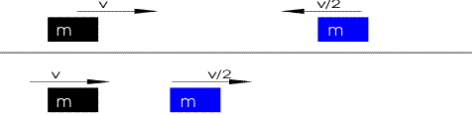
\includegraphics[scale=.6]{pic1.png}
	\newline
	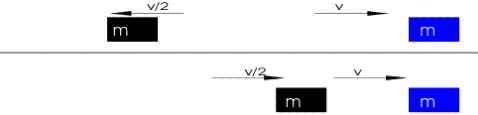
\includegraphics[scale=.6]{pic2.png}
	
	\end{figure}
	
	It is worth noting that this will not be entirely accurate when the objects do not collide in a head-on fashion. This will be corrected in further implementations.\newline  
	
	Profiling reveals this area of the implementation as a  computational hotspot as the problem size increases. This is due to a number of expensive operations (multiplication and square root) being called for each unique pairing of objects.\newline
	
	This can be approximated as $!n \times t$ calls for each operation where $n$ is the number of objects and $t$ is the number of time steps.  \newline
	
	%------------------------------------------------
	
	\section{Verification}
	
	The following steps have been taken to verify the implementation:
	
	\begin{itemize}
		\item Check functionality at small object and time step values
		\item Print all position and velocity values into a file and manually check physics.
		\item Print all collisions and related object information into file upon occurance
	\end{itemize}

	As discussed briefly in the previous section, the collision physics used in the collision handling will not be valid for angled collisions. This will be corrected in future implementations by separating collision logic into head collisions and angled collisions.\newline
	
	In future revisions, object positions may be visualised with an external program to further verify correctness.
		
	%------------------------------------------------
	
	\section{Serial Performance}
	Results of performance scaling with problem size can be seen in table 1. \newline
	\begin{table}
		\caption{Performance over problem size}
		\centering
		\begin{tabular}{llr}
			\toprule
			\multicolumn{2}{c}{Problem size} \\
			\cmidrule(r){1-2}
			Num. Objects & Num Timesteps & Run Time (s) \\
			\midrule
			50 & 20 & $< 0.000001$ \\
			500 & 20 & $0.05$ \\
			1000 & 20 & $0.28$ \\
			5000 & 20 & $5.50$ \\
			10000 & 20 & $19.80$ \\
			500 & 100 & $0.21$ \\
			1000 & 100 & $0.70$ \\
			5000 & 100 & $13.86$ \\
			10000 & 100 & $45.00$ \\
			500 & 500 & $2.16$ \\
			1000 & 500 & $7.16$ \\
			5000 & 500 & $130$ \\
			500 & 1000 & $4.40$ \\
			500 & 5000 & $20.30$ \\
			\bottomrule
		\end{tabular}
	\end{table}	
	
	%----------------------------------------------------------------------------------------
	%	REFERENCE LIST
	%----------------------------------------------------------------------------------------
	
	\begin{thebibliography}{99} % Bibliography - this is intentionally simple in this template
		
		\bibitem[S. Steinmann, 2006]{gif:1}
		Steinmann, S., (2006).
		\newblock {\em Elastic collision of masses in a system with a moving frame of reference}
		\newline Accessed from URL:\newline $https://en.wikipedia.org/wiki/Elastic\_collision$
		
	\end{thebibliography}
	
	%----------------------------------------------------------------------------------------
	
\end{document}\documentclass{article}
